\documentclass{beamer}


%********** beamer settings **********
\usetheme{Madrid} %{default} %{Singapore} %{Warsaw} %{Copenhagen} %{Madrid}
%\setbeamertemplate{navigation symbols}{} % remove the navigation symbols
%\useoutertheme{infolines} % use outer theme for footer.
%\setbeamercolor{normal text}{bg=red!12} % set background color
%\setbeamercolor{normal text}{bg=mybackground} % set background color

%********** fonts settings **********
\usepackage{fontspec,xunicode,xltxtra}
\setmainfont{Times New Roman}
\setsansfont{Arial} % beamer默认使用sans font
%\setmonofont{Source Sans Pro}

%********** new fonts commands **********
%\newfontfamily\SourceSansPro{Source Sans Pro}

%********** Chinese fonts input **********
\usepackage{xeCJK}
\setCJKmainfont{宋体}
\setCJKsansfont{宋体}
\setCJKmonofont{宋体}
\XeTeXlinebreaklocale "zh"
\XeTeXlinebreakskip=0pt plus 1pt minus 0.1pt

%********** using packages **********
\usepackage{metalogo} % for XeTeX, XeLaTeX logo
\usepackage{listings} % for listing source code
% listings settings
\lstset{
  language=C,
  numbers=left,
  numberstyle=\scriptsize,
  frame=leftline,
  xleftmargin=1em,
  flexiblecolumns=false,
  basicstyle=\ttfamily\small,
  breaklines=true,
  extendedchars=true,
  escapechar=\%,
  texcl=true,
  showstringspaces=false,
  %keywordstyle=\bfseries,
  keywordstyle=\color{cyan},
  commentstyle=\tiny\color{blue}\slshape,
  tabsize=4
}

%********** colors and drawing pictures **********
%\usepackage{xcolor} % beamer 自动加载xcolor
\usepackage{graphicx}
\usepackage{fancybox}

%********** Misc **********
\usepackage{verbatim}
%%% for bookmarks
\usepackage{hyperref}
%********** hyperref settings **********
\hypersetup{
  bookmarksnumbered=true,
  bookmarksopen=true,
  pdfborder=1,
  breaklinks,
  colorlinks,
  linkcolor=cyan,
  filecolor=black,
  urlcolor=blue,
  citecolor=green
}




\usepackage{xcolor}
\colorlet{HEADCOLOR}{red!50}
\colorlet{BRANCHCOLOR}{blue!50}
\colorlet{WORKCOLOR}{gray!50}
\colorlet{INDEXCOLOR}{cyan!50}
\colorlet{COMMITCOLOR}{green!50}

\usepackage{tikz}
\usetikzlibrary{shapes,arrows,positioning,calc,backgrounds,matrix,fit}
\tikzset{
  basic-style/.style = {
    rectangle, rounded corners=2pt, draw, thick,
    fill=#1,
    minimum height=15pt,
    minimum width=1.4cm,
    inner sep=1pt
  },
  commit-style/.style = {
    basic-style=COMMITCOLOR
  },
  index-style/.style = {
    basic-style=INDEXCOLOR,
    minimum width=2.5cm
  },
  work-style/.style = {
    basic-style=WORKCOLOR,
    minimum width=2.5cm
  },
  branch-style/.style = {
    basic-style=BRANCHCOLOR
  },
  head-style/.style = {
    basic-style=HEADCOLOR
  },
  cmd-style/.style = {
    #1=5pt
  },
  cmd-style/.default = right,
  main-style/.style = {
    execute at end picture = {
      \begin{pgfonlayer}{background}
        \path[fill=gray!20,rounded corners]
          ([xshift=-0.2cm,yshift=-0.2cm]current bounding box.south west) rectangle
          ([xshift=0.2cm,yshift=0.2cm]current bounding box.north east);
          %(current bounding box.south west) rectangle
          %  (current bounding box.north east);
        \end{pgfonlayer}
    }
  },
  file-style/.style = {
    draw=red, fill=yellow!30, inner sep=2pt
  },
  dir-style/.style = {
    fill=green!50,inner sep=2pt
  },
  dir-bg-style/.style = {
    fill=cyan!30,rounded corners
  },
  every edge/.style = {draw, ->, >=latex', thick}
}

%%%%% new definitions %%%%%

\newlength\commitDistance
\setlength\commitDistance{0.5cm}
\newlength\indexWorkDistance
\setlength\indexWorkDistance{2\commitDistance}

\newcommand\displayName[1]{\ttfamily\bfseries #1}
\newcommand\commandName[1]{\ttfamily\bfseries\small #1}

\def\createNode style:#1 name:#2 display:#3 direct:#4 distance:#5 to:#6;{
  \node [#1, #4=#5 of #6] (#2) {#3}
        edge [#4] (#6);
}
\def\createCommit name:#1 display:#2 direct:#3 to:#4;{
  \node [commit-style, #3=\commitDistance of #4] (#1) {#2}
        edge [#3, COMMITCOLOR] (#4);
}
\def\createBranch name:#1 display:#2 direct:#3 to:#4;{
  \node [branch-style, #3=0.75\commitDistance of #4] (#1) {#2}
        edge [#3, BRANCHCOLOR] (#4);
}
\def\createHead direct:#1 to:#2;{
  \node [head-style, #1=0cm of #2] (head) {HEAD};
}
\def\createIndex to:#1;{
  \node [index-style, below=2\commitDistance of #1] (index) {Index};
}
\def\createWork to:#1;{
  \node [work-style, below=2\commitDistance of #1] (work) {Work DIR};
}

\newcommand\makeOutline{
  %\useasboundingbox (-0.1,-3.6) rectangle (10.7,2);
  \node[right] (dumy) at (0,0) {\dots};
  \createCommit name:a display:{\displayName A} direct:right to:dumy;
  \createCommit name:b display:{\displayName B} direct:right to:a;
  \createCommit name:c display:{\displayName C} direct:right to:b;
  \createCommit name:d display:{\displayName D} direct:right to:c;
  \createCommit name:e display:{\displayName E} direct:right to:d;

  \createIndex to:c;
  \createWork to:index;
}

\newcommand\createMatrix[2]{
  \matrix [
    matrix of nodes,
    nodes={rectangle,draw=red,fill=yellow!30,minimum width=1.3cm,font=\ttfamily\small,inner sep=2pt},
    row sep=-\pgflinewidth,
    column sep=-\pgflinewidth,
  ] (m#1) at #2 {
    \textcolor{blue}{list-#1}\\
    a.h\\
    b.h\\
    c.h\\
    $d_{v#1}.h$\\
  };
}

\newcommand\createHashMatrix[2]{
  \matrix [
    matrix of nodes,
    nodes={rectangle,draw=red,fill=yellow!30,minimum width=1.3cm,font=\ttfamily\small,inner sep=2pt},
    row sep=-\pgflinewidth,
    column sep=-\pgflinewidth,
  ] (m#1) at #2 {
    \textcolor{blue}{hash-#1}\\
    a47c3\\
    b325c\\
    c10b9\\
    \textcolor{cyan}{da98#1}\\
  };
}

\usepackage{calc} % for \real control sequence
%%%%%%%%%%%%%%%%%%%%%
\newlength {\boxw}
\newlength {\boxh}
\newlength {\boxd}
\newlength {\boxroundness}
\newlength {\boxshadowsize}
\newlength {\shadowiter}
\newlength {\innersep}


\setlength {\boxshadowsize}{6pt}
\setlength {\boxroundness}{3pt}

\newsavebox {\shadowblockbox}
\newenvironment{shadowblock}[4] % {minipage width}{fill color}{draw color}{inner sep}
{\def\fillcolor{#2}\def\drawcolor{#3}%
  \setlength {\innersep}{#4}%
  \begin{lrbox}{\shadowblockbox}\begin{minipage}{#1}}
{\end{minipage}\end{lrbox}
  % draw the textbox
  \settowidth {\boxw}{\usebox{\shadowblockbox}}   % get box's width
  \settoheight {\boxh}{\usebox{\shadowblockbox}}  % get box's height
  \settodepth {\boxd}{\usebox{\shadowblockbox}}   % get box's depth

  \addtolength {\boxh}{\boxd}
  \addtolength {\boxw}{2\boxroundness}
  \addtolength {\boxh}{2\boxroundness}
  \addtolength {\boxw}{2\innersep}
  \addtolength {\boxh}{2\innersep}
  
  \begin{tikzpicture}
    % draw the shadow
    \foreach \x in {0,0.05,...,1} {
      \setlength{\shadowiter}{\boxshadowsize*\real{\x}}
      \fill[xshift=\boxshadowsize-1pt,yshift=-\boxshadowsize+1pt,
          black,opacity=0.04,rounded corners=\boxroundness]
          (\shadowiter,\shadowiter) rectangle +(\boxw-2\shadowiter,\boxh-2\shadowiter);
    }
    % draw the box border
    \filldraw[fill=\fillcolor,draw=\drawcolor,rounded corners=\boxroundness]
        (0,0) rectangle (\boxw,\boxh);
    % draw the content
    \node[xshift=\boxroundness,yshift=\boxroundness,inner sep=\innersep,outer sep=0pt,anchor=south west]
        at (0,0) {\usebox{\shadowblockbox}};
  \end{tikzpicture}
}

\newcommand\gitcmd[1]{%
%\begin{center}
%  \noindent\fcolorbox{white}{yellow!20}{%
%    \begin{minipage}{.7\textwidth}
%      \centering\Large
%      \texttt{#1}
%    \end{minipage}}
%\end{center}

\begin{center}
  \begin{shadowblock}{0.7\textwidth}{yellow!50}{black!50}{0pt}
  \centering\Large
  \texttt{#1}
  \end{shadowblock}
\end{center}
}

%\newsavebox{\framedtextbox}
%\newenvironment{framedtext}[1] % minipage width
%{\begin{lrbox}{\framedtextbox}\begin{minipage}{#1}\centering}
%{\end{minipage}\end{lrbox}
%  % put box in a tikz node, and draw the node.
%  \begin{tikzpicture}
%    \node [fill=gray!20,rounded corners] at (0,0) {\usebox{\framedtextbox}};
%  \end{tikzpicture}
%}
\newenvironment{framedtext}
{\begin{center}\begin{shadowblock}{0.7\textwidth}{gray!20}{red}{10pt}}
{\end{shadowblock}\end{center}}

\newcommand\surrounded[1]{
  \textless #1\textgreater
}

\newcommand\optionalSurrounded[1]{
  [\textless #1\textgreater]
}


%********** title page settings **********
\title{Using GIT}
\author{孙延宾}
\institute{西安$\cdot$业务软件开发一部$\cdot$~\texttt{ZTE}}
\date{\today}

\begin{document}

%*************** title page *****************
\begin{frame}[plain]
  \titlepage
\end{frame}
%*************** title page *****************

%%%%%%%%%%%%%%%%%%%%% Introduce %%%%%%%%%%%%%%%%%%%%%%%%%%
\part[What is git]{What is git}
\begin{frame}
\begin{framedtext}
  什么是Git?\\[1em]
  Git是一个分布式版本控制软件,是Linux内核之父Linus Torvalds为了更好地管理Linux内核开发而创立的。
\end{framedtext}
\end{frame}

\begin{frame}
\begin{framedtext}
  如何理解Git?\\[1em]
  想象一下,在任何版本控制软件出现以前,人们是如何管理软件开发的呢?或许,最简单的方法就是“复制”、“粘贴”。
\end{framedtext}
\end{frame}

\begin{frame}{copy working directory as a version}
\begin{center}
  \begin{tikzpicture}%[main-style]
    %%% directory - 1
    \node[file-style] (a1) {\tiny a.h};
    \node[file-style,right=0.2cm of a1] (b1) {\tiny b.h};
    \node[file-style,right=0.2cm of b1] (c1) {\tiny c.h};
    \node[file-style,below=0.1cm of b1] (d1) {\tiny\textcolor{blue}{$d_{v1}.h$}};
    \node[dir-style,below=0.2cm of d1] (dir1) {\tiny directory-1};
    \begin{pgfonlayer}{background}
      \node [dir-bg-style,fit=(a1) (b1) (c1) (d1) (dir1)] {};
    \end{pgfonlayer}

    %%% directory - 2
    \node[file-style,right=1.5cm of c1] (a2) {\tiny a.h};
    \node[file-style,right=0.2cm of a2] (b2) {\tiny b.h};
    \node[file-style,right=0.2cm of b2] (c2) {\tiny c.h};
    \node[file-style,below=0.1cm of b2] (d2) {\tiny\textcolor{blue}{$d_{v2}.h$}};
    \node[dir-style,below=0.2cm of d2] (dir2) {\tiny directory-2};
    \begin{pgfonlayer}{background}
      \node [dir-bg-style,fit=(a2) (b2) (c2) (d2) (dir2)] {};
    \end{pgfonlayer}

    %%% directory - 3
    \node[file-style,right=1.5cm of c2] (a3) {\tiny a.h};
    \node[file-style,right=0.2cm of a3] (b3) {\tiny b.h};
    \node[file-style,right=0.2cm of b3] (c3) {\tiny c.h};
    \node[file-style,below=0.1cm of b3] (d3) {\tiny\textcolor{blue}{$d_{v3}.h$}};
    \node[dir-style,below=0.2cm of d3] (dir3) {\tiny directory-3};
    \begin{pgfonlayer}{background}
      \node [dir-bg-style,fit=(a3) (b3) (c3) (d3) (dir3)] {};
    \end{pgfonlayer}

    %%% working directory
    \node[file-style,below=2cm of dir2] (b4) {\tiny b.h};
    \node[file-style,left=0.2cm of b4] (a4) {\tiny a.h};
    \node[file-style,right=0.2cm of b4] (c4) {\tiny c.h};
    \node[file-style,below=0.1cm of b4] (d4) {\tiny $d_{v3}.h$};
    \node[dir-style,below=0.2cm of d4] (dir4) {\tiny working dir};
    \begin{pgfonlayer}{background}
      \node [dir-bg-style,fit=(a4) (b4) (c4) (d4) (dir4)] {};
    \end{pgfonlayer}

    %%% arrows
    % dir-1 to dir2
    \path[->] ([xshift=1cm]d1.east) edge ([xshift=-1cm]d2.west);
    % dir-2 to dir3
    \path[->] ([xshift=1cm]d2.east) edge ([xshift=-1cm]d3.west);
    % working dir to dir1
    \path[->] ([yshift=0.2cm]a4.north west) edge node[right]{\tiny copy as v1} ([yshift=-0.2cm]dir1.south);
    % working dir to dir2
    \path[->] ([yshift=0.2cm]b4.north) edge node[right]{\tiny copy as v2} ([yshift=-0.2cm]dir2.south);
    % working dir to dir3
    \path[->] ([yshift=0.2cm]c4.north east) edge node[right]{\tiny copy as v3} ([yshift=-0.2cm]dir3.south);
  \end{tikzpicture}
\end{center}
\end{frame}

\begin{frame}
\begin{framedtext}
  文件冗余?\\[1em]
  显然,很多文件没有改动却被复制了很多次,为此考虑单独创建一个目录放置文件,每一个版本用“文件列表”来代替。
\end{framedtext}
\end{frame}

\begin{frame}{put all files in a repository directory}
\begin{center}
  \begin{tikzpicture}
    %%% file lists
    \createMatrix{1}{(0,0)}
    \createMatrix{2}{([xshift=3cm]m1)}
    \createMatrix{3}{([xshift=3cm]m2)}

    %%% repository
    \node[file-style,above=2.5cm of m2] (bRepo) {\tiny b.h};
    \node[file-style,left=0.2cm of bRepo] (aRepo) {\tiny a.h};
    \node[file-style,right=0.2cm of bRepo] (cRepo) {\tiny c.h};
    \node[file-style,below=0.1cm of bRepo] (dRepoV1) {\tiny $d_{v1}.h$};
    \node[file-style,below=0.1cm of dRepoV1] (dRepoV2) {\tiny $d_{v2}.h$};
    \node[file-style,below=0.1cm of dRepoV2] (dRepoV3) {\tiny $d_{v3}.h$};
    \node[dir-style,below=0.2cm of dRepoV3] (dirRepo) {\tiny repository dir};
    \begin{pgfonlayer}{background}
      \node [dir-bg-style,fit=(aRepo) (bRepo) (cRepo) (dRepoV1) (dRepoV2) (dRepoV3) (dirRepo)] {};
    \end{pgfonlayer}

    %%% working directory
    \node[file-style,below=1cm of m2] (bWork) {\tiny b.h};
    \node[file-style,left=0.2cm of bWork] (aWork) {\tiny a.h};
    \node[file-style,right=0.2cm of bWork] (cWork) {\tiny c.h};
    \node[file-style,below=0.1cm of bWork] (dWork) {\tiny $d_{v3}.h$};
    \node[dir-style,below=0.2cm of dWork] (dirWork) {\tiny working dir};
    \begin{pgfonlayer}{background}
      \node [dir-bg-style,fit=(aWork) (bWork) (cWork) (dWork) (dirWork)] {};
    \end{pgfonlayer}

    %%% arrows
    \path[->] (m1.east) edge (m2.west);
    \path[->] (m2.east) edge (m3.west);
  \end{tikzpicture}
\end{center}
\end{frame}

\begin{frame}
\begin{framedtext}
  文件名并不是一个好方法!\\[1em]
  通过修改文件名来区分一个文件的不同版本,显然不是一个好方法,为此,将“文件内容”映射到SHA1字符串,
  用这些SHA1字符串来区分文件的不同版本。同一个文件的不同版本,只跟文件内容相关。
\end{framedtext}
\end{frame}

\begin{frame}{map file content to SHA-1 string}
\begin{center}
  \begin{tikzpicture}
    %%% file lists
    \createHashMatrix{1}{(0,0)}
    \createHashMatrix{2}{([xshift=3cm]m1)}
    \createHashMatrix{3}{([xshift=3cm]m2)}

    %%% repository
    \node[file-style,above=2.5cm of m2] (bRepo) {\tiny b325c};
    \node[file-style,left=0.2cm of bRepo] (aRepo) {\tiny a47c3};
    \node[file-style,right=0.2cm of bRepo] (cRepo) {\tiny c10b9};
    \node[file-style,below=0.1cm of bRepo] (dRepoV1) {\tiny da981};
    \node[file-style,below=0.1cm of dRepoV1] (dRepoV2) {\tiny da982};
    \node[file-style,below=0.1cm of dRepoV2] (dRepoV3) {\tiny da983};
    \node[dir-style,below=0.2cm of dRepoV3] (dirRepo) {\tiny repository dir};
    \begin{pgfonlayer}{background}
      \node [dir-bg-style,fit=(aRepo) (bRepo) (cRepo) (dRepoV1) (dRepoV2) (dRepoV3) (dirRepo)] {};
    \end{pgfonlayer}

    %%% working directory
    \node[file-style,below=1cm of m2] (bWork) {\tiny b.h};
    \node[file-style,left=0.2cm of bWork] (aWork) {\tiny a.h};
    \node[file-style,right=0.2cm of bWork] (cWork) {\tiny c.h};
    \node[file-style,below=0.1cm of bWork] (dWork) {\tiny d.h};
    \node[dir-style,below=0.2cm of dWork] (dirWork) {\tiny working dir};
    \begin{pgfonlayer}{background}
      \node [dir-bg-style,fit=(aWork) (bWork) (cWork) (dWork) (dirWork)] {};
    \end{pgfonlayer}

    %%% arrows
    \path[->] (m1.east) edge (m2.west);
    \path[->] (m2.east) edge (m3.west);
  \end{tikzpicture}
\end{center}
\end{frame}

\begin{frame}
\begin{framedtext}
  添加一个缓存文件列表!\\[1em]
  当文件数量很多时(如Linux kernel),遍历所有文件是一件很耗时的事情。
  为此添加一个缓存文件,保存所有改动
  过的文件列表,当创建新的版本时,上一个版本的文件列表与缓存文件列表比较,
  即可得到新版本的文件列表。
\end{framedtext}
\end{frame}

\begin{frame}{add an index file}
\begin{center}
  \begin{tikzpicture}
    %%% file lists
    \createHashMatrix{1}{(0,0)}
    \createHashMatrix{2}{([xshift=3cm]m1)}
    \createHashMatrix{3}{([xshift=3cm]m2)}

    %%% repository
    \node[file-style,above=2cm of m2] (bRepo) {\tiny b325c};
    \node[file-style,left=0.2cm of bRepo] (aRepo) {\tiny a47c3};
    \node[file-style,right=0.2cm of bRepo] (cRepo) {\tiny c10b9};
    \node[file-style,below=0.1cm of bRepo] (dRepoV1) {\tiny da981};
    \node[file-style,below=0.1cm of dRepoV1] (dRepoV2) {\tiny da982};
    \node[file-style,below=0.1cm of dRepoV2] (dRepoV3) {\tiny da983};
    \node[dir-style,below=0.2cm of dRepoV3] (dirRepo) {\tiny repository dir};
    \begin{pgfonlayer}{background}
      \node [dir-bg-style,fit=(aRepo) (bRepo) (cRepo) (dRepoV1) (dRepoV2) (dRepoV3) (dirRepo)] {};
    \end{pgfonlayer}

    \matrix [
      matrix of nodes,
      nodes={rectangle,draw=red,fill=yellow!30,minimum width=1.3cm,font=\ttfamily\tiny,inner sep=2pt},
      row sep=-\pgflinewidth,
      column sep=-\pgflinewidth,
      below=-0.1cm of m2
    ] (index){
      \textcolor{blue}{index}\\
      a47c3: a.h\\
      b325c: b.h\\
      c10b9: c.h\\
      da983: d.h\\
    };

    %%% working directory
    \node[file-style,below=0.1cm of index] (bWork) {\tiny b.h};
    \node[file-style,left=0.2cm of bWork] (aWork) {\tiny a.h};
    \node[file-style,right=0.2cm of bWork] (cWork) {\tiny c.h};
    \node[file-style,below=0.1cm of bWork] (dWork) {\tiny d.h};
    \node[dir-style,below=0.1cm of dWork] (dirWork) {\tiny working dir};
    \begin{pgfonlayer}{background}
      \node [dir-bg-style,fit=(aWork) (bWork) (cWork) (dWork) (dirWork)] {};
    \end{pgfonlayer}

    %%% arrows
    \path[->] (m1.east) edge (m2.west);
    \path[->] (m2.east) edge (m3.west);
    \path[->,dashed] (cWork.east) edge[bend right=45] (index-4-1.east);
    \path[->,dashed] ([yshift=0.05cm]index-4-1.east) edge[out=0,in=180] (m3-4-1);
    \path[->,dashed] (m3-4-1.east) edge[out=30,in=-10] (cRepo.east);
  \end{tikzpicture}
\end{center}
\end{frame}

\begin{frame}
\begin{framedtext}
%  这就是Git!\\[1em]
%  保存文件的目录对应于Git的本地仓库;\\
%  每个版本的文件列表对应于Git的commit;\\
%  缓存文件列表对应于Git的index文件;\\
%  工作目录对应于Git的工作目录。

  这就是Git!\\[1em]
  \begin{tabular}{rcl}
    保存文件的目录 & : & git repository \\
    版本文件列表 & : & git commit \\
    缓存文件列表 & : & git index \\
    工作目录 & : & git work dir
  \end{tabular}
\end{framedtext}
\end{frame}

\begin{frame}
\begin{center}
\begin{tikzpicture}[main-style]
    \makeOutline
    \createBranch name:release display:{\displayName release} direct:above to:b;
    \createBranch name:master display:{\displayName master} direct:above to:e;
    \createHead direct:above to:master;

    \createIndex to:c;
    \createWork to:index;
\end{tikzpicture}
\end{center}
\end{frame}

%%%%%%%%%%%%%%%%%%%%% Local Operation %%%%%%%%%%%%%%%%%%%%%%%%
\part[Local Operations]{Local Operations}
\begin{frame}
\begin{center}
  \ttfamily\huge
  Git的本地操作
\end{center}
\end{frame}

\section[git add]{git add}
\begin{frame}{\ {}}
  \gitcmd{git add}
\end{frame}

\begin{frame}{git add}
\begin{center}
  \begin{tikzpicture}[main-style]
    \makeOutline
    \createBranch name:release display:{\displayName release} direct:above to:b;
    \createBranch name:master display:{\displayName master} direct:above to:e;
    \createHead direct:above to:master;

    \createIndex to:c;
    \createWork to:index;

    \path (work) edge[bend right=30] node[cmd-style=left]{\commandName git add files/directories} (index);
  \end{tikzpicture}
\end{center}
\end{frame}

\section[git commit]{git commit}
\begin{frame}{\ {}}
  \gitcmd{git commit}
\end{frame}

\begin{frame}{git commit}
\begin{center}
  \begin{tikzpicture}[main-style]
    \makeOutline
    \createBranch name:release display:{\displayName release} direct:above to:b;
    \createBranch name:master display:{\displayName master} direct:above to:e;
    \createHead direct:above to:master;

    \createIndex to:c;
    \createWork to:index;

    \path (index) edge[out=60,in=245] node[cmd-style=below,near end]{\commandName git commit} (e);
  \end{tikzpicture}
\end{center}
\end{frame}

\section[git checkout]{git checkout}
\begin{frame}{\ {}}
  \gitcmd{git checkout}
\end{frame}
\begin{frame}{git checkout}
\begin{center}
  \begin{tikzpicture}[main-style]
    \makeOutline
    \createBranch name:release display:{\displayName release} direct:above to:b;
    \createBranch name:master display:{\displayName master} direct:above to:e;
    \createHead direct:above to:master;

    \createIndex to:c;
    \createWork to:index;

    \path (index) edge[bend right=30] node[cmd-style=left]{\commandName git checkout -- files} (work);
    \path (e.south) edge[bend left=45] node[circle,fill=red,swap,auto,inner sep=1pt] {\tiny{1}}
      node[cmd-style=left,swap,pos=0.15]{\commandName git checkout E} (index.east);
    \path (e.south) edge[bend left=45]
      node[circle,fill=red,auto,swap,inner sep=1pt] {\tiny{2}} (work.east);
  \end{tikzpicture}
\end{center}
\end{frame}

\section[git reset]{git reset}
\begin{frame}{\ {}}
  \gitcmd{git reset}
\end{frame}

\subsection[git reset \texttt{-{}-} files]{git reset \texttt{-{}-} files}
\begin{frame}{\ {}}
  \gitcmd{git reset \texttt{-{}-} files}
\end{frame}

\begin{frame}{git reset \texttt{-{}-} files}
\begin{center}
  \begin{tikzpicture}[main-style]
    \makeOutline
    \createBranch name:release display:{\displayName release} direct:above to:b;
    \createBranch name:master display:{\displayName master} direct:above to:e;
    \createHead direct:above to:master;

    \createIndex to:c;
    \createWork to:index;

    \path (e.south) edge[out=270,in=0] node[cmd-style=above,auto,swap]{\commandName git reset -- files} (index.east);
  \end{tikzpicture}
\end{center}
\end{frame}

\subsection[git reset \texttt{-{}-}soft commit]{git reset \texttt{-{}-}soft commit}
\begin{frame}{\ {}}
  \gitcmd{git reset \texttt{-{}-}soft commit}
\end{frame}

\begin{frame}{git reset \texttt{-{}-}soft commit}
\begin{center}
  \begin{tikzpicture}[main-style]
    \makeOutline
    \createBranch name:release display:{\displayName release} direct:above to:b;

    % create old master branch & HEAD
    \path <1> node [branch-style, above=0.75\commitDistance of e] (master) {master}
        edge [cmd-style, BRANCHCOLOR] (e);
    % create new master branch & HEAD
    \path <2> node [branch-style, above=0.75\commitDistance of d] (master) {master}
        edge [cmd-style, BRANCHCOLOR] (d);
    \path <2-> (e.north west) edge[bend right=30,<->] (d.north east);
    \createHead direct:above to:master;

    \createIndex to:c;
    \createWork to:index;
  \end{tikzpicture}
\end{center}
\end{frame}

\subsection[git reset \texttt{-{}-}mixed commit]{git reset \texttt{-{}-}mixed commit}
\begin{frame}{\ {}}
  \gitcmd{git reset \texttt{-{}-}mixed commit}
\end{frame}

\begin{frame}{git reset \texttt{-{}-}mixed commit}
\begin{center}
  \begin{tikzpicture}[main-style]
    \makeOutline
    \createBranch name:release display:{\displayName release} direct:above to:b;

    % create old master branch & HEAD
    \path <1> node [branch-style, above=0.75\commitDistance of e] (master) {master}
        edge [cmd-style, BRANCHCOLOR] (e);
    % create new master branch & HEAD
    \path <2-> node [branch-style, above=0.75\commitDistance of d] (master) {master}
        edge [cmd-style, BRANCHCOLOR] (d);
    \path <2-> (e.north west) edge[bend right=30,<->] node[circle,above,auto,swap,fill=red,inner sep=1pt]{\tiny{1}}
                (d.north east);
    \createHead direct:above to:master;

    \createIndex to:c;
    \createWork to:index;

    \path <3-> (e.south) edge[bend left=45] node[circle,fill=red,swap,auto,inner sep=1pt] {\tiny{2}}(index.east);
  \end{tikzpicture}
\end{center}
\end{frame}

\subsection[git reset \texttt{-{}-}hard commit]{git reset \texttt{-{}-}hard commit}
\begin{frame}{\ {}}
  \gitcmd{git reset \texttt{-{}-}hard commit}
\end{frame}

\begin{frame}{git reset \texttt{-{}-}hard commit}
\begin{center}
  \begin{tikzpicture}[main-style]
    \makeOutline
    \createBranch name:release display:{\displayName release} direct:above to:b;

    % create old master branch & HEAD
    \path <1> node [branch-style, above=0.75\commitDistance of e] (master) {master}
        edge [cmd-style, BRANCHCOLOR] (e);
    % create new master branch & HEAD
    \path <2-> node [branch-style, above=0.75\commitDistance of d] (master) {master}
        edge [cmd-style, BRANCHCOLOR] (d);
    \path <2-> (e.north west) edge[bend right=30,<->] node[circle,above,auto,swap,fill=red,inner sep=1pt]{\tiny{1}}
                (d.north east);
    \createHead direct:above to:master;

    \createIndex to:c;
    \createWork to:index;

    \path <3-> (e.south) edge[bend left=45] node[circle,fill=red,swap,auto,inner sep=1pt] {\tiny{2}}(index.east);
    \path <4-> (e.south) edge[bend left=45]
      node[circle,fill=red,auto,swap,inner sep=1pt] {\tiny{3}} (work.east);
  \end{tikzpicture}
\end{center}
\end{frame}

\section[git diff]{git diff}
\begin{frame}{\ {}}
  \gitcmd{git diff}
\end{frame}

\begin{frame}{git diff}
\begin{center}
  \begin{tikzpicture}[main-style]
    \makeOutline
    \createBranch name:release display:{\displayName release} direct:above to:a;
    \createBranch name:master display:{\displayName master} direct:above to:e;
    \createHead direct:above to:master;

    \createIndex to:c;
    \createWork to:index;

    \path <1-> (work.north west) edge[bend left=45,<->] node[left]{\displayName git diff file} (index.south west);
    \path <2-> (index.east) edge[bend right=45,<->] node[above,auto,near end]{\displayName git diff --cached file} (e.south);
    \path <3-> (work.east) edge[bend right=45,<->] node[above,auto,pos=0.4]{\displayName git diff E file} (e.-70);
    \path <4-> (b.north east) edge[bend left=30,<->] node[above,auto]{\displayName git diff B..D file} (d.north west);
  \end{tikzpicture}
\end{center}
\end{frame}


\section[git branch]{git branch}
\begin{frame}{\ {}}
  \gitcmd{git branch}
\end{frame}

\begin{frame}{git branch}
\begin{framedtext}
  \small
  本质上来说,git没有“分支”的概念。所谓的分支,其实就是commit的别名,
  一个分支(如master)对应到一个文件(如refs/head/master),该文件中
  保存着一个commit-id,分支类似于C语言中的指针。\\[10pt]
  \textcolor{blue}{分支是廉价的}。\\[10pt]
  请使用develop、release分支,拒绝锁流。
\end{framedtext}
\end{frame}

\begin{frame}{show branch names}
\gitcmd{
  git branch [-r] [-a]
}
\begin{center}
{\ttfamily\small
\begin{tabular}{rcl}
    no option & : & 列出本地所有分支 \\
    -r & : & 列出远程仓库中的所有分支 \\
    -a & : & 列出本地、远程的所有分支 \\
  \end{tabular}
}
\end{center}
\end{frame}

\begin{frame}{create new branch}
\gitcmd{\small
  git branch \surrounded{new-branch} \optionalSurrounded{based-commit}
}
\begin{center}
{\ttfamily\small
  基于\optionalSurrounded{based-commit}创建新分支\surrounded{new-branch}。\\
  如果\optionalSurrounded{based-commit}被省略,则基于HEAD创建新分支。
}
\end{center}
\end{frame}


%%% branch operations
\section[git merge]{git merge}
\begin{frame}{\ {}}
  \gitcmd{git merge}
\end{frame}

\begin{frame}{git merge}
\begin{center}
  \begin{tikzpicture}

  \end{tikzpicture}
\end{center}
\end{frame}


\section[git rebase]{git rebase}
\begin{frame}{\ {}}
  \gitcmd{git rebase}
\end{frame}

\begin{frame}{git rebase}
\begin{center}
  \begin{tikzpicture}

  \end{tikzpicture}
\end{center}
\end{frame}


%%%%%%%%%%%%%%%%%% Remote Operations %%%%%%%%%%%%%%%%%%%%%%
\part[Remote Operations]{Remote Operations}
\begin{frame}
\begin{center}
  \ttfamily\huge
  Git的远程操作
\end{center}
\end{frame}

\section[git remote]{git remote}
\begin{frame}{\ {}}
\gitcmd{
  git remote show \surrounded{repo-name}
}
\end{frame}
\begin{frame}{show information of remote repo \texttt{origin}}
\begin{framedtext}
{
  e.g.\\[5pt]
  git remote show \textbf{origin}
}
\end{framedtext}
\end{frame}
\begin{frame}{output of \texttt{git remote show origin}}
  \textcolor{blue!50}{\ttfamily Output:}
  \lstinputlisting{remoteshow.txt}
\end{frame}


\section[git fetch]{git fetch}
\begin{frame}{\ {}}
\gitcmd{\small
  git fetch [\surrounded{repo-name} [\surrounded{rbranch:lbranch}]]
}
\begin{center}
{\small\ttfamily
  \begin{tabular}{rcl}
    \multicolumn{3}{l}{将远程仓库代码拉取到本地。} \\[10pt]
    repo-name & : & 远程仓库名称,如origin \\
    rbranch   & : & 远程分支 \\
    lbranch   & : & 本地分支 \\
  \end{tabular}
}
\end{center}
\end{frame}


\section[git pull]{git pull}
\begin{frame}{\ {}}
\gitcmd{git pull}
\begin{center}
  \begin{minipage}{0.7\textwidth}
    \ttfamily
    pull等价于fetch + merge,先拉取代码,然后合入当前分支。
  \end{minipage}
\end{center}
\end{frame}


\section[git push]{git push}
\begin{frame}{\ {}}
\gitcmd{git push}
\centerline{将代码从本地仓库推送到远程仓库,支持默认值设置。}
\end{frame}

\begin{frame}{git push configuration}
\gitcmd{\small
  \begin{tabular}{rr}
    \multicolumn{2}{l}{git config --global push.default}\\
    \  & nothing|matching|upstream|simple|current \\
  \end{tabular}
}
\begin{center}
{\small\ttfamily
  \begin{tabular}{rcl}
    nothing & : & 顾名思义\\
    matching& : & push所有与远程分支同名(匹配)\\
            &   & 的本地分支\\
    upstream& : & push所有pull下来的分支\\
    simple  & : & 类似于upstream,但是要求远程、\\
            &   & 本地分支同名\\
    current & : & push当前分支\\
  \end{tabular}
}
\end{center}
\end{frame}


%%%%%%%%%%%%%%%%%% Tips and Tricks %%%%%%%%%%%%%%%%%%%%%%%%
\part[Tips and Tricks]{Tips and Tricks}
\begin{frame}
\begin{center}
  \ttfamily\huge
  Git常用技巧
\end{center}
\end{frame}

\section[fetch a single branch]{fetch a single branch}
\begin{frame}{fetch a single branch}

\gitcmd{\small\ttfamily
  \begin{tabular}{rl}
    git clone & --single-branch\\
              & --branch\surrounded{rbranch} \ --depth 1\\
              & \surrounded{repo-url} \optionalSurrounded{directory}
  \end{tabular}
}
\begin{center}
{\ttfamily
  \begin{tabular}{rcl}
    --single-branch&:&只复制一个分支\\
    --branch\surrounded{rbranch}&:&分支名称,并将HEAD指向该分支\\
    --depth 1&:&只复制最新的1个commit\\
  \end{tabular}
}
\end{center}
\end{frame}

\section[apply a patch]{apply a patch}
\begin{frame}{create patch files 1}
  \gitcmd{\normalsize git diff > filename.[patch|diff]}
\vspace{1em}
\begin{center}
\begin{minipage}{0.7\textwidth}
  \ttfamily
  该方法使用“标准”的diff格式创建patch文件,
  该patch文件在Git, SVN, BitKeeper等工具上
  都可以使用。
\end{minipage}
\end{center}
\end{frame}

\begin{frame}{create patch files 2}
  \gitcmd{\normalsize git format-patch \surrounded{commit-id}}
\vspace{1em}
\begin{center}
\begin{minipage}{0.7\textwidth}
  \ttfamily
  从\surrounded{commit-id}(不包括该commit)到HEAD之间的
  每个commit生成一个patch文件。
  注意,这样生成的patch文件只适用于Git。
\end{minipage}
\end{center}
\end{frame}

\begin{frame}{apply patch file}
  \gitcmd{\small\ttfamily
    \begin{tabular}{rl}
      git apply & [--stat | --summary |\\
                & \ --check | --reverse]\\
                & filename.[diff | patch]\\
    \end{tabular}
  }
\begin{center}
{\ttfamily
  \begin{tabular}{rcl}
    --stat&:&只输出统计信息而不应用补丁内容\\
    --summary&:&显示补丁摘要\\
    --check&:&检查是否能成功的应用该补丁的内容\\
    --reverse&:&将应用过的补丁内容撤销\\
  \end{tabular}
}
\end{center}
\end{frame}

\section[special signs]{special signs}
\begin{frame}{special signs}
\gitcmd{\small
  \begin{tabular}{rcl}
    \^ & : & 第一个parent commit \\
       &   & e.g. HEAD\^{}2: second parent commit \\[10pt]
    \~ & : & 第一个upstream commit \\
       &   & e.g. HEAD\~{}2: parent's parent commit\\
  \end{tabular}
}
\end{frame}

\section[show branch topology]{show branch topology}
\begin{frame}{show branch topology}
  \gitcmd{git show-branch}
\end{frame}

\begin{frame}{show branch topology cont.}
  \textcolor{blue!50}{\ttfamily Output:}
  \lstinputlisting{showbranch.txt}
\end{frame}

\section[git GUI]{git GUI}
\begin{frame}{Git GUI}
\gitcmd{git gui}
\end{frame}

\begin{frame}{Git GUI cont.}
\begin{figure}
  \centering
  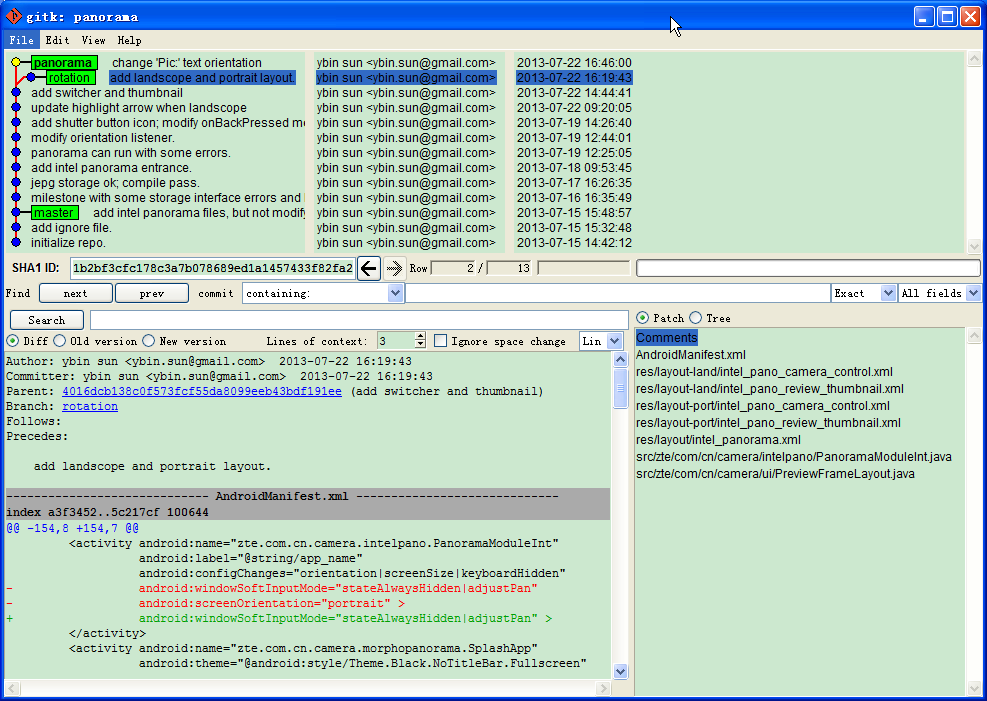
\includegraphics[width=0.8\textwidth]{gitk.png}%\\
  %\caption{GUI Window}\label{fig:gitk}
\end{figure}
\end{frame}

\section[external diff tool]{external diff tool}
\begin{frame}{external tools configuration}
\gitcmd{\small
  \begin{tabular}{rl}
    git config & \texttt{--}global \\
               & external.diff diff\_4\_git.bat \\[5pt]
    %git config & \texttt{--}blobal \\
    %           & external.merge merge\_4\_git.bat \\
  \end{tabular}
}
\end{frame}

\begin{frame}{external diff tool}
  \textcolor{blue!50}{\ttfamily cat diff\_4\_git.bat}
  \lstinputlisting{diff.bat}
\end{frame}


\section[git log]{git log}
\begin{frame}{git log}
\gitcmd{\normalsize\ttfamily
  \begin{flushleft}
    git log\\
    查看完整历史记录\\[8pt]
    git log \surrounded{filename}\\
    查看\surrounded{filename}的完整历史记录\\[8pt]
    git log \surrounded{commit-id}\\
    查看从\surrounded{commit-id}开始的历史记录\\[8pt]
    git log \surrounded{commit-id} \surrounded{filename}\\
    查看从\surrounded{commit-id}开始的\surrounded{filename}\\
    的历史记录
  \end{flushleft}
}
\end{frame}


\section[show index file]{show index file}
\begin{frame}{show index file}
  \gitcmd{git ls-files --stage}
\end{frame}

\begin{frame}{show index file cont.}
\begin{figure}
  \centering
  % Requires \usepackage{graphicx}
  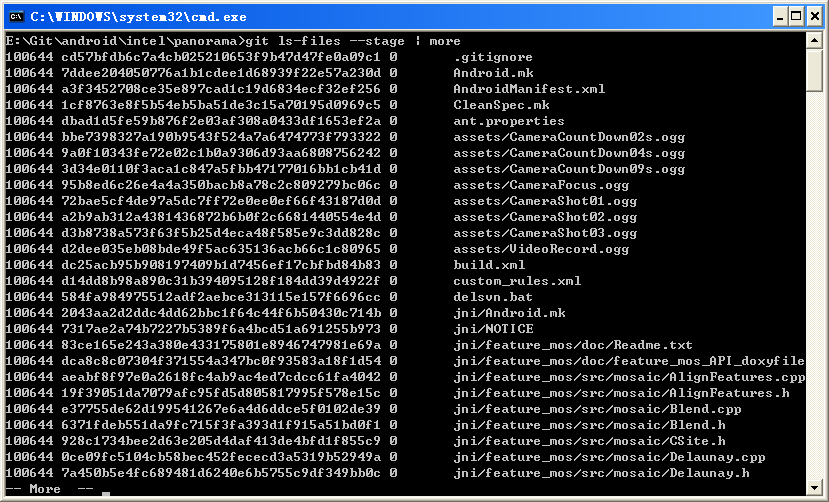
\includegraphics[width=0.8\textwidth]{showindex.png}%\\
  %\caption{show index content}\label{fig:showindex}
\end{figure}
\end{frame}

\section[git add]{git add}
\begin{frame}{git add}
\gitcmd{\normalsize
  git add [--update] [--all] filename/dir
}
\end{frame}

\begin{frame}[fragile]{git add cont.}
\begin{center}
\begin{tikzpicture}
  \matrix [
    matrix of nodes,
    nodes={rectangle,draw=red,fill=yellow!30,minimum width=3cm,minimum height=20pt,font=\ttfamily\Large},
    row sep=-\pgflinewidth,
    column sep=-\pgflinewidth,
    text depth=0.5ex, % WTF
    text height=2ex,  % and this.
  ] (gitadd){
    new & modified & deleted\\
  };
  \draw[decorate,decoration={brace,raise=5pt,amplitude=10pt},draw=cyan,thick]
    (gitadd-1-1.north west) -- (gitadd-1-3.north east) node[midway,above=15pt]{\ttfamily --all};

  \draw[decorate,decoration={brace,mirror,raise=2pt,amplitude=10pt},draw=green,thick]
    (gitadd-1-1.south west) -- (gitadd-1-2.south east) node[midway,below=15pt]{\ttfamily no options};

  \draw[decorate,decoration={brace,mirror,raise=5pt,amplitude=10pt},draw=blue,thick]
    (gitadd-1-2.south west) -- (gitadd-1-3.south east) node[midway,below=15pt]{\ttfamily --update};
\end{tikzpicture}
\end{center}
\end{frame}

\section[online repository]{online repository}
\begin{frame}{online repository}
\gitcmd{\normalsize
  \begin{tabular}{rcl}
    国外站点 & : & https://github.com\\
             &   & https://bitbucket.org\\
    国内站点 & : & https://git.oschina.net\\
             &   & https://code.csdn.net\\
             &   & https://gitcafe.com\\
  \end{tabular}
}
\end{frame}
\begin{frame}{online repository cont.}
\begin{framedtext}
{
  e.g.\\[5pt]
  git clone https://github.com/ybin/tex.git
}
\end{framedtext}
\end{frame}

\section[git vs repo]{git vs repo}
\begin{frame}{git vs repo}
\begin{framedtext}
{
  \textcolor{blue}{\emph{repo}}是Google为管理Android源码而创建的工具。
  由于Android源码极其庞大,不得不将其分解为多个独立的
  git项目,如Camera, Music, Video Player等,这就需要
  一个工具来“统一”管理这些git项目,于是便有了repo。repo
  并非独立的工具,它以git作为其后端。
}
\end{framedtext}
\end{frame}

\part[\surrounded{/end}]{\surrounded{/end}}
\begin{frame}{\surrounded{/end}}
  \begin{framedtext}
    \begin{tabular}{ll}
      \textcolor{blue}{weibo} & @iGNU \\
      \textcolor{blue}{email} & ybin.sun@gmail.com \\
      \textcolor{blue}{github}& https://github.com/\textbf{ybin}/ \\
    \end{tabular}
  \end{framedtext}
\end{frame}


\end{document}
